\chapter{Solution Architecture}
\label{chap:architecture}

% =====================================================================
%  Chapter 3 with glossary/acronym cross-references wired in.
%  Acronyms: \gls{} on first prose use (auto-expands), \acrshort{} in
%  tables (short form, no expansion). Glossary terms: \gls{} / \glsdisp{}.
%  Requires the entries from chap3-additions.tex to be present in
%  acronimos.tex and glossario.tex, otherwise these keys are undefined.
% =====================================================================

This chapter describes the architecture of the proposed tool. It presents the two complementary analyses the tool performs, the shared vocabulary that ties their results together, the decomposition into components, the data that moves between them, and the architectural decisions that a reviewer is most likely to question. Implementation detail, meaning how each component is actually built, is deferred to Chapter~\ref{chap:implementation}; this chapter stays at the level of structure and rationale.

\section{Overview}

The tool answers a single question, ``how secure is this \gls{mcp} server,'' along two paths that are useful in different situations. The first is a \emph{dynamic} analysis: it connects to a running server, reasons about the tools the server exposes, and sends real attack traffic to find out which of those tools actually leak or misbehave. The second is a \emph{static} analysis: it reads a server's source code and flags the code that would answer those same attacks, without connecting to anything or executing a single line.

The two paths are deliberately built on one foundation. Both label every finding with the same vulnerability taxonomy (Section~\ref{sec:taxonomy}) and draw remediation text from the same catalog. A finding of type \texttt{command\_injection} therefore means the same thing whether it came from a payload that succeeded against a live server or from a line of source code that a parser flagged. This shared vocabulary is what lets a developer fix statically what the dynamic path would otherwise prove the hard way, and it is the single most important structural property of the design.

\section{The Dynamic Scan Pipeline}
\label{sec:pipeline}

The dynamic path is a seven-step pipeline, shown in Figure~\ref{fig:pipeline}. The steps fall into two groups separated by a human decision, and that separation is a security property of the architecture rather than a convenience of the user interface.

\begin{figure}[htbp]
    \centering
    % TODO: export images/arch-pipeline.svg to images/arch-pipeline.pdf
    % (Overleaf: upload the .svg and it is converted on compile; locally use
    %  Inkscape or rsvg-convert. The .svg source is already in images/.)
    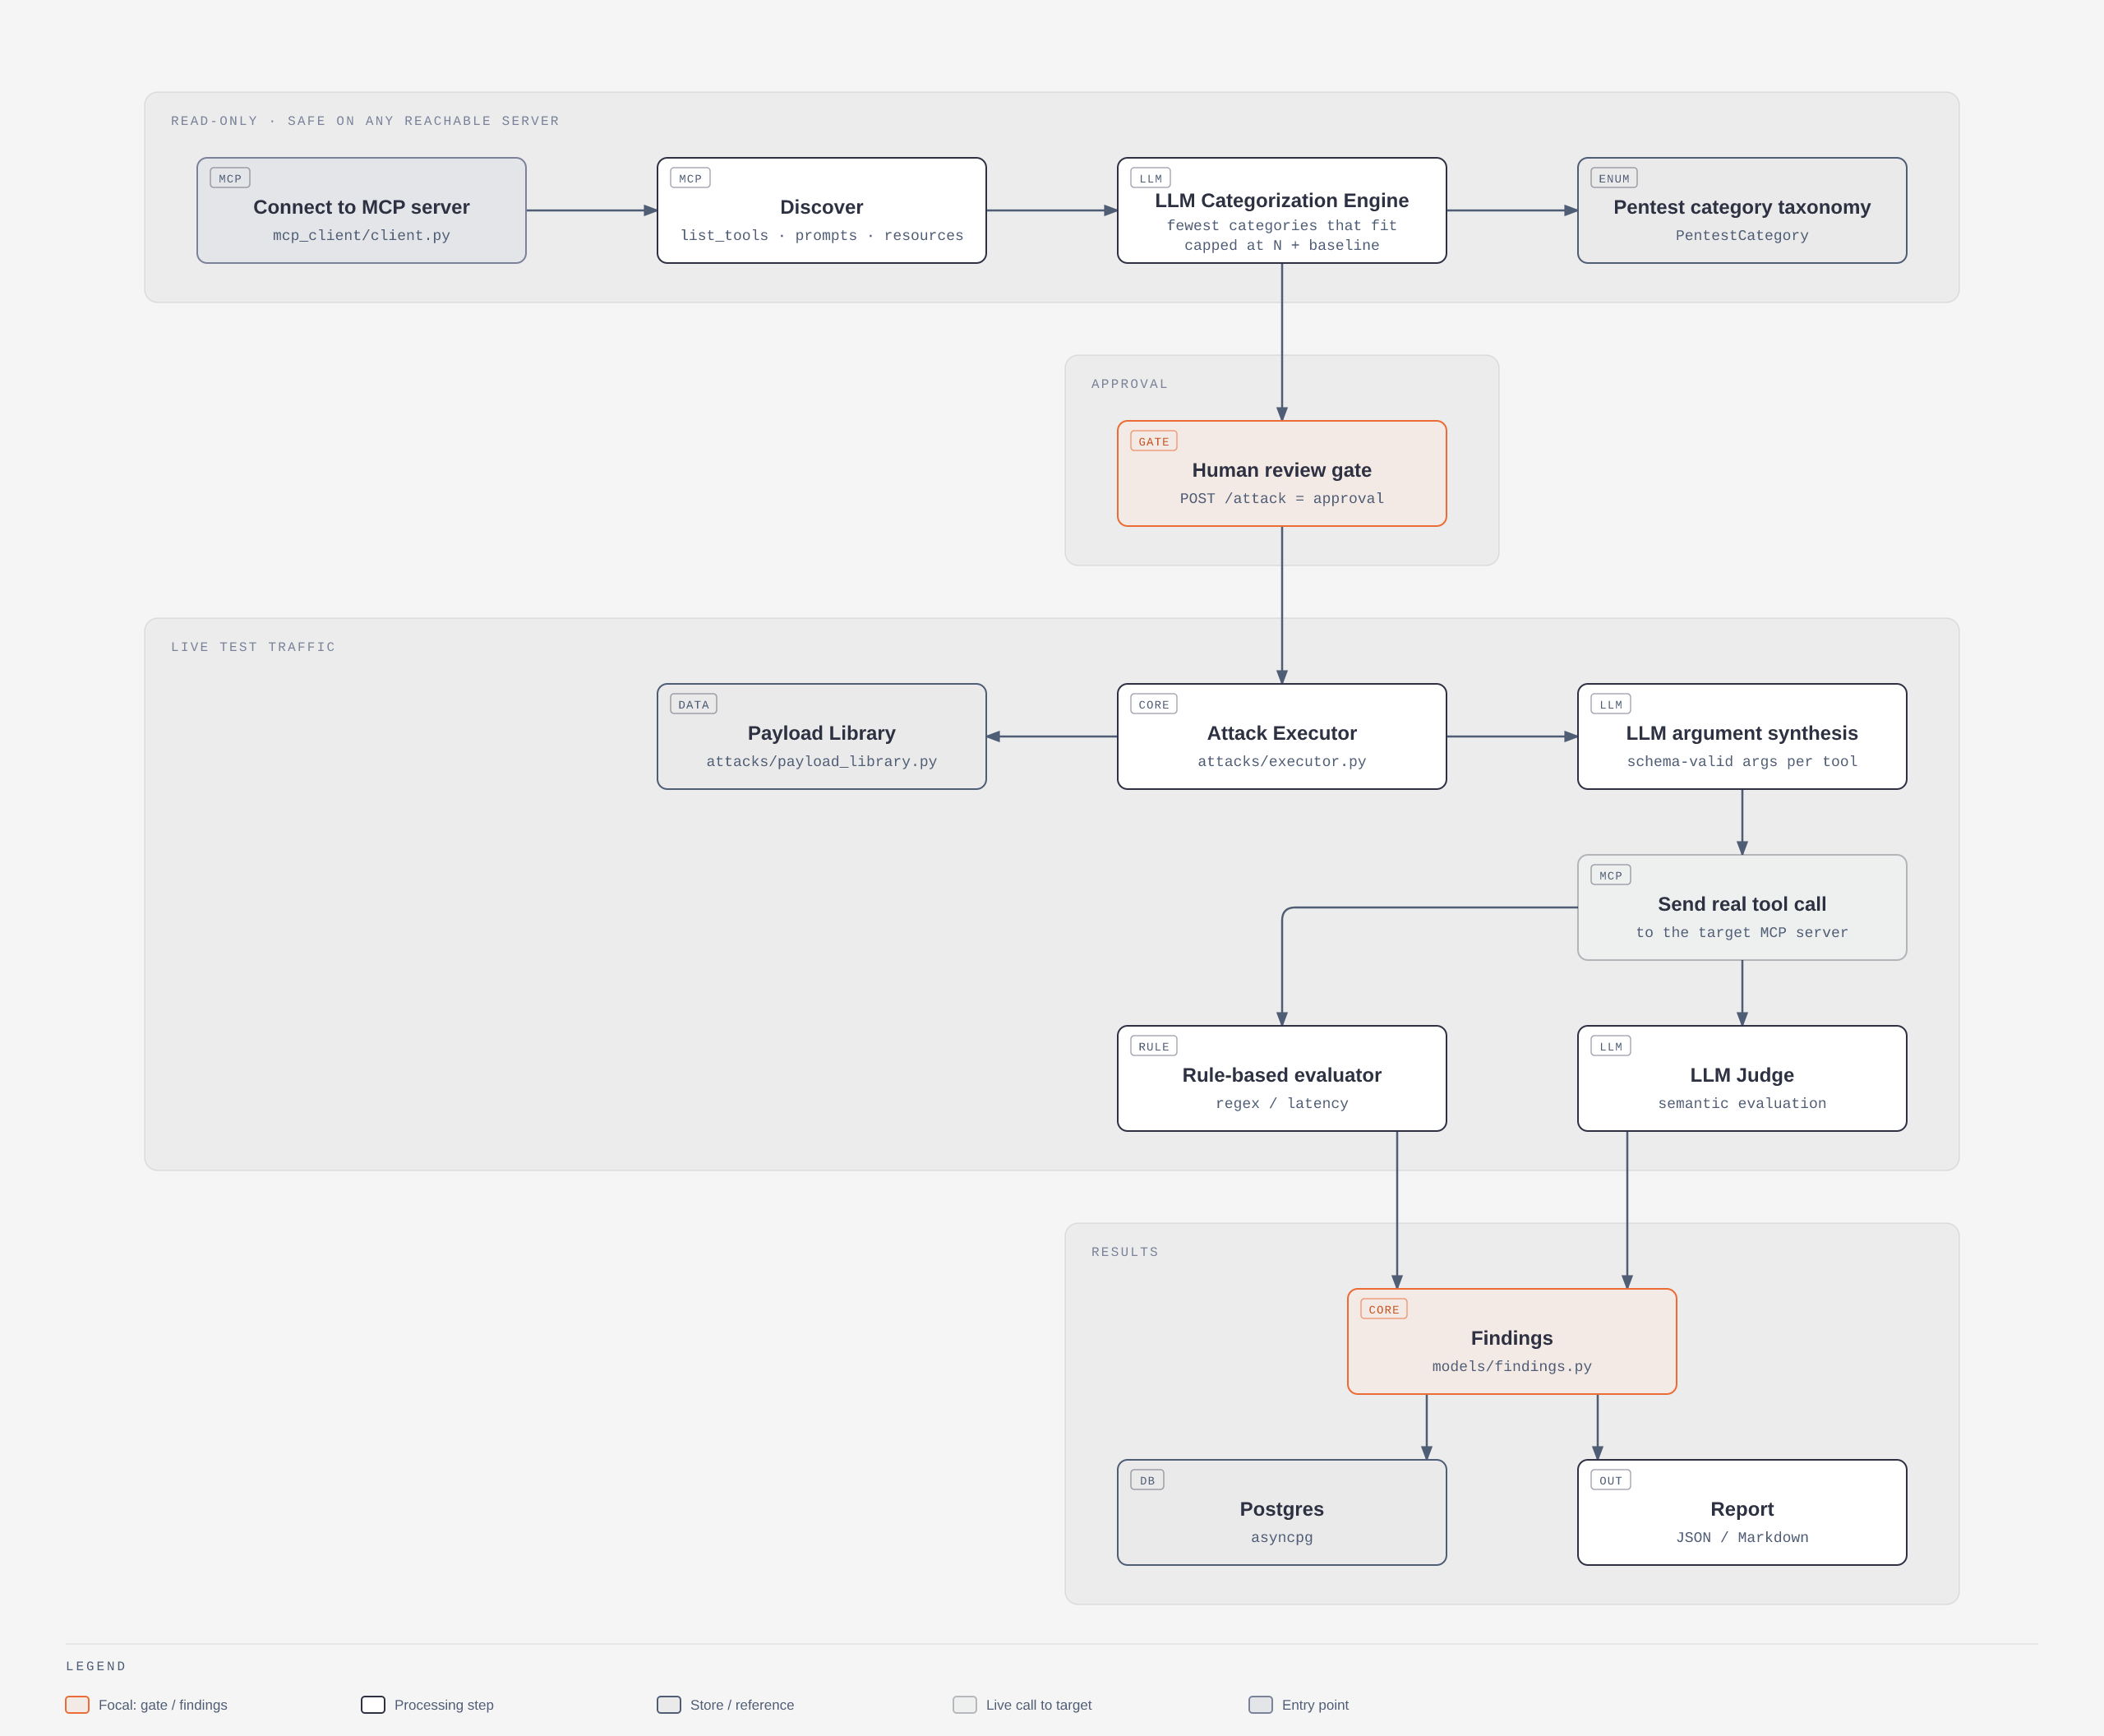
\includegraphics[width=\linewidth]{images/arch-pipeline.png}
    \caption{The dynamic scan pipeline. Steps 1--3 are read-only; steps 5--7 send live attack traffic and run only after an explicit approval.}
    \label{fig:pipeline}
\end{figure}

The first group discovers and understands the target without touching it in anger. The tool connects to the \gls{mcp} server over one of the protocol's transports, calls the server's own listing methods to enumerate the tools, prompts, and resources it exposes, and then classifies each discovered tool. Classification is where a language model first enters the pipeline. A System One model, Jev (Section~\ref{sec:system-one}), reads each tool's name, description, and input schema and answers one independent yes/no question per category, returning the probability that the category is the tool's primary attack surface. The application keeps only the categories above a probability threshold, at most one per tool in the current configuration, so a plainly database-backed tool is not tagged with a spread of speculative categories that would each multiply the attacks sent. Everything up to this point is read-only and safe to run against any reachable server.

Between understanding and attacking sits a \glsdisp{human_in_the_loop}{human-in-the-loop} gate. The categorization is returned to the operator for inspection, and nothing is attacked until the operator explicitly approves. This gate is not cosmetic: it is the boundary at which the tool stops being an observer and starts sending traffic that could cause real effects, and the architecture makes that boundary an explicit, separate action.

The second group tests and reports. For each approved combination of tool, category, and payload, the \gls{llm} synthesizes a schema-valid call that places the attack \gls{payload} in the field most likely to reach a vulnerable \gls{sink} while filling every other required field with a plausible benign value. Each response is then evaluated twice. Fast deterministic rules catch known-format leaks such as secrets, stack traces, or \glsdisp{canary_string}{canary strings}, and an \gls{llm} judge catches the leaks that only semantic understanding can recognize, such as a response that returned another tenant's record. The judge is required to quote the exact span of the response that proves the leak, and the tool verifies that quote is present before trusting the verdict. Finally, the confirmed findings are assembled into a structured report. Each finding carries a \gls{cvss} v3.1 base score and severity band, its impact on confidentiality, integrity, and availability, the judge's confidence, the evidence, and the exact payload used.

\newpage

\section{Vulnerability Taxonomy}
\label{sec:taxonomy}

The taxonomy is the shared vocabulary named in the overview. It extends a small set of initial categories into a fuller set aligned with the \gls{owasp} Top 10 for \gls{llm} Applications and the MITRE \gls{atlas} mappings established in the project's earlier research phase, so a finding here cites the same external framing used elsewhere. Table~\ref{tab:taxonomy} lists the categories and what each one looks for.

\begin{table}[htbp]
\centering
\small
\begin{tabular}{p{4.2cm} p{8.0cm}}
\hline
\textbf{Category} & \textbf{What it looks for} \\
\hline
\acrshort{sql} Injection & Parameters that build or forward a database query \\
\gls{command_injection} & Parameters that reach a shell or subprocess \\
\gls{path_traversal} & File-path parameters on read/write/list/delete tools \\
\acrshort{ssrf} & \acrshort{url} or host parameters that trigger outbound requests \\
Information Extraction & Responses containing secrets, credentials, or internal metadata \\
Resource Extraction & Over-broad or cross-tenant resource exposure \\
\gls{jailbreak} / \gls{prompt_injection} & Tools that process natural-language or instruction text \\
Auth \& Access Control & Privileged-sounding tools, tested under a low-privilege session \\
\glsdisp{deserialization_attack}{Deserialization} & Parameters parsed as \acrshort{json}, \acrshort{yaml}, or pickled data \\
Memory \& Persistence Poisoning & Writes to stores read back in a different session \\
\acrshort{dos} / Resource Exhaustion & Unbounded or expensive operations \\
Generic Schema \glsdisp{fuzzing}{Fuzzing} & Applied to every tool as the baseline floor \\
\hline
\end{tabular}
\caption{The pentest category taxonomy shared by the dynamic and static paths.}
\label{tab:taxonomy}
\end{table}

One category, generic schema fuzzing, is a non-negotiable floor. Every tool receives it regardless of what the classifier decides, which matters because a tool description is untrusted content that an attacker could craft to talk the classifier out of flagging anything. The floor guarantees that every tool is attacked at a baseline level even if the classifier is manipulated, fails, or times out. The rationale for this floor as a defense against injection aimed at the tool's own triage step is examined in Section~\ref{sec:decisions}.

\subsection{Severity Scoring}
\label{sec:scoring}

A finding has to say how serious it is and what it puts at risk. Rather than define a project-specific scale, the tool adopts the \gls{cvss} v3.1 base metrics~\cite{first2019cvss}. The choice has two practical consequences. First, the confidentiality, integrity, and availability triad is already part of every \gls{cvss} vector as the C, I, and A impact metrics, so the \gls{cia} impact of a finding is read directly from the same vector that produces its score. Second, the 0 to 10 number and its band (None, Low, Medium, High, Critical) are computed by the standard's published formula, so no score in the report is chosen by hand.

Each category in the taxonomy is assigned one base vector, stored next to its remediation text in the shared catalog. All vectors assume an \gls{mcp} server reachable over the network by an unauthenticated caller (AV:N, PR:N, UI:N) unless the category itself implies otherwise. Table~\ref{tab:cvss} lists the vectors and the resulting scores.

\begin{table}[htbp]
\centering
\small
\begin{tabular}{p{4.0cm} p{4.6cm} c c c}
\hline
\textbf{Category} & \textbf{Base vector (after \texttt{CVSS:3.1/})} & \textbf{Score} & \textbf{Band} & \textbf{C/I/A} \\
\hline
Command Injection & \texttt{AV:N/AC:L/PR:N/UI:N/S:C/C:H/I:H/A:H} & 10.0 & Critical & H/H/H \\
SQL Injection & \texttt{AV:N/AC:L/PR:N/UI:N/S:U/C:H/I:H/A:L} & 9.4 & Critical & H/H/L \\
SSRF & \texttt{AV:N/AC:L/PR:N/UI:N/S:C/C:H/I:L/A:N} & 9.3 & Critical & H/L/N \\
Jailbreak / Prompt Injection & \texttt{AV:N/AC:L/PR:N/UI:N/S:C/C:L/I:H/A:N} & 9.3 & Critical & L/H/N \\
Memory \& Persistence Poisoning & \texttt{AV:N/AC:L/PR:N/UI:N/S:C/C:L/I:H/A:N} & 9.3 & Critical & L/H/N \\
Path Traversal & \texttt{AV:N/AC:L/PR:N/UI:N/S:U/C:H/I:L/A:N} & 8.2 & High & H/L/N \\
Auth \& Access Control & \texttt{AV:N/AC:L/PR:L/UI:N/S:U/C:H/I:H/A:N} & 8.1 & High & H/H/N \\
Deserialization & \texttt{AV:N/AC:H/PR:N/UI:N/S:U/C:H/I:H/A:H} & 8.1 & High & H/H/H \\
Information Extraction & \texttt{AV:N/AC:L/PR:N/UI:N/S:U/C:H/I:N/A:N} & 7.5 & High & H/N/N \\
DoS / Resource Exhaustion & \texttt{AV:N/AC:L/PR:N/UI:N/S:U/C:N/I:N/A:H} & 7.5 & High & N/N/H \\
Resource Extraction & \texttt{AV:N/AC:L/PR:L/UI:N/S:U/C:H/I:N/A:N} & 6.5 & Medium & H/N/N \\
Generic Schema Fuzzing & \texttt{AV:N/AC:L/PR:N/UI:N/S:U/C:N/I:L/A:L} & 6.5 & Medium & N/L/L \\
\hline
\end{tabular}
\caption{\gls{cvss} v3.1 base vector, score, band, and \gls{cia} impact per taxonomy category.}
\label{tab:cvss}
\end{table}

The metric choices that move the score most deserve a justification. Scope is set to changed (S:C) where a successful attack reaches a component beyond the \gls{mcp} server itself: command injection escapes into the host operating system, \gls{ssrf} reaches internal services behind the server, and prompt injection and memory poisoning alter the behaviour of the \gls{llm} agent that consumes the tool's output. Availability is high (A:H) for resource exhaustion, whose whole effect is denial of service, and for command injection and deserialization, where arbitrary code execution can stop the process. Deserialization is the only category with high attack complexity (AC:H), because exploiting it generally requires a gadget chain that matches the target's libraries; this is why it scores below path traversal despite a high impact on all three properties. Resource extraction and access-control failures require low privileges (PR:L), since both describe an authenticated caller reaching data beyond its own. Generic schema fuzzing carries only low integrity and availability impact, because a fuzzing hit shows that malformed input is mishandled but does not by itself demonstrate a leak.

These vectors are a defensible starting point, not fixed truths, and they are kept as data in the catalog so they can be revised without touching code.


\section{The Static Analysis Path}
\label{sec:static}

The static path reads source code and never connects to a server. It walks a checkout for Python files, parses each one, inventories what the server exposes, and flags the code an attacker could reach. The inventory records server instantiation, the tool, resource, and prompt registrations with their parameters and line ranges, the declared transport, and any authentication hints. Risk detection then runs over the same files and keeps only the findings that map onto the taxonomy, attributing each one to the specific tool whose body contains it. A dangerous call inside a registered tool is reachable by anything that can invoke that tool; the same call in a helper script is not, and the attribution preserves that distinction.

The two paths exist together because they answer different questions about the same weakness, as Table~\ref{tab:static-vs-dynamic} sets out. The static path answers ``which code would answer this payload,'' with a line of source as evidence, before the dynamic path, or anyone else's pentest tool, answers ``did this payload actually work'' with the server's response as evidence.

\begin{table}[htbp]
\centering
\small
\begin{tabular}{p{3.2cm} p{4.6cm} p{4.6cm}}
\hline
 & \textbf{Dynamic scan} & \textbf{Static analysis} \\
\hline
Needs & Running server and credentials & A source checkout \\
Sends attack traffic & Yes, after the human gate & Never \\
Answers & ``Did this payload work?'' & ``Which code answers it?'' \\
Evidence & The server's response & The line of code \\
\hline
\end{tabular}
\caption{The two analysis paths answer different questions over the same taxonomy.}
\label{tab:static-vs-dynamic}
\end{table}

\section{Component Architecture}
\label{sec:components}

Figure~\ref{fig:components} shows the decomposition into components. At the centre is a set of data models that form the shared vocabulary every other component speaks: a normalized representation of a discovered tool, the categorization result, the synthesized attacks and their verdicts, and the final report. Keeping these models in one place is what allows the dynamic and static paths to produce comparable output without coordinating directly.

\begin{figure}[htbp]
    \centering
    % TODO: export images/arch-components.svg to images/arch-components.pdf
    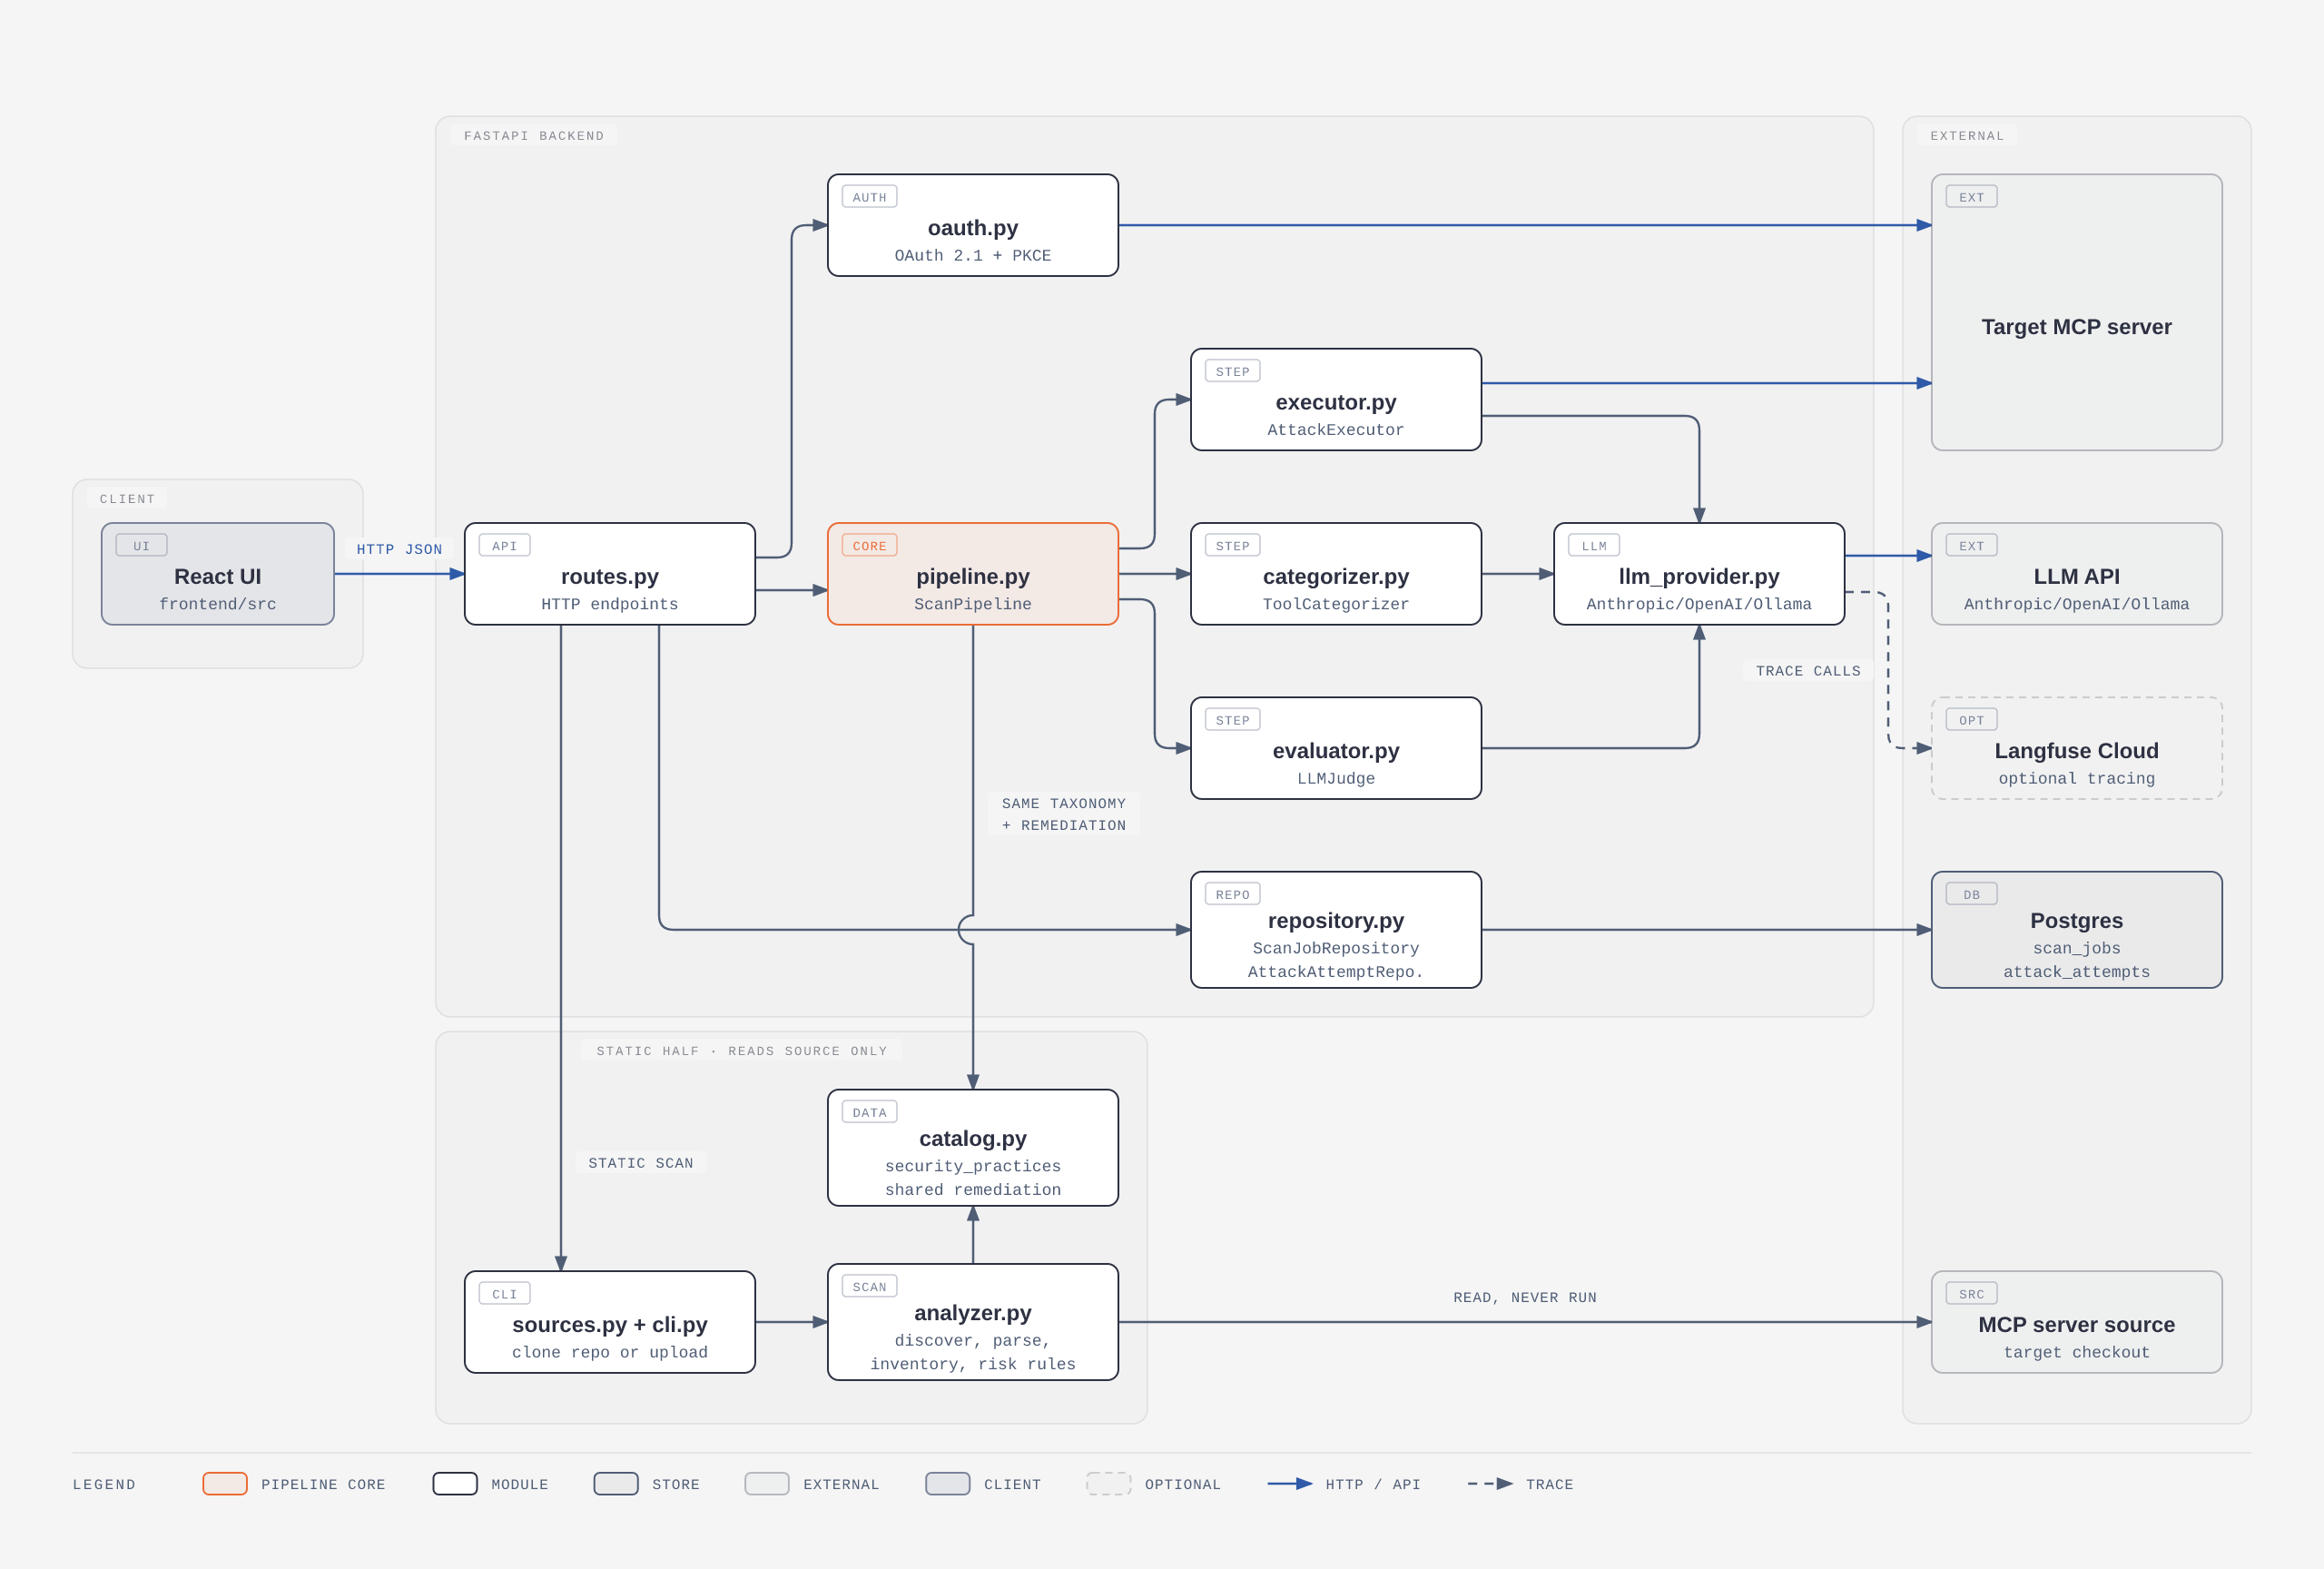
\includegraphics[width=\linewidth]{images/arch-components.png}
    \caption{Component decomposition. The shared data models sit between the two analysis paths.}
    \label{fig:components}
\end{figure}

Around that core, the dynamic path is built from an \gls{mcp} client that handles the three transports, a connection layer that owns credential lifecycle and the \gls{oauth} flow, a categorization component that calls the Jev \gls{api}, an \gls{llm} provider component shared by attack synthesis and judging, an attacks component that holds the payload library and the synthesis logic, an evaluation component that runs the dual verdict, and an orchestration layer that wires these together and owns the human-approval split. The static path is a self-contained set of components for obtaining source, walking it safely, parsing it, inventorying the exposed surface, and running the risk rules. Supporting both are a security-practices catalog that supplies remediation, a persistence layer that is the only code allowed to touch the database, a reporting component, and the web \gls{api}. A React frontend presents the whole as three tabs: the live-scan wizard, the payload library and attack history, and the code-review view.

\section{Data Model and Persistence}
\label{sec:data}

Figure~\ref{fig:data-model} shows the persisted data model. The design records the \emph{outputs} of a scan, the snapshot of what the server exposed, the categorization, and the report, and stores them in a relational database using \acrshort{json} columns so that these evolving structures do not require a rigid schema this early in the project. Durable scan history is what gives the tool value a single-shot scanner lacks: the ability to compare a server against itself over time.

\begin{figure}[htbp]
    \centering
    % TODO: export images/arch-data-model.svg to images/arch-data-model.pdf
    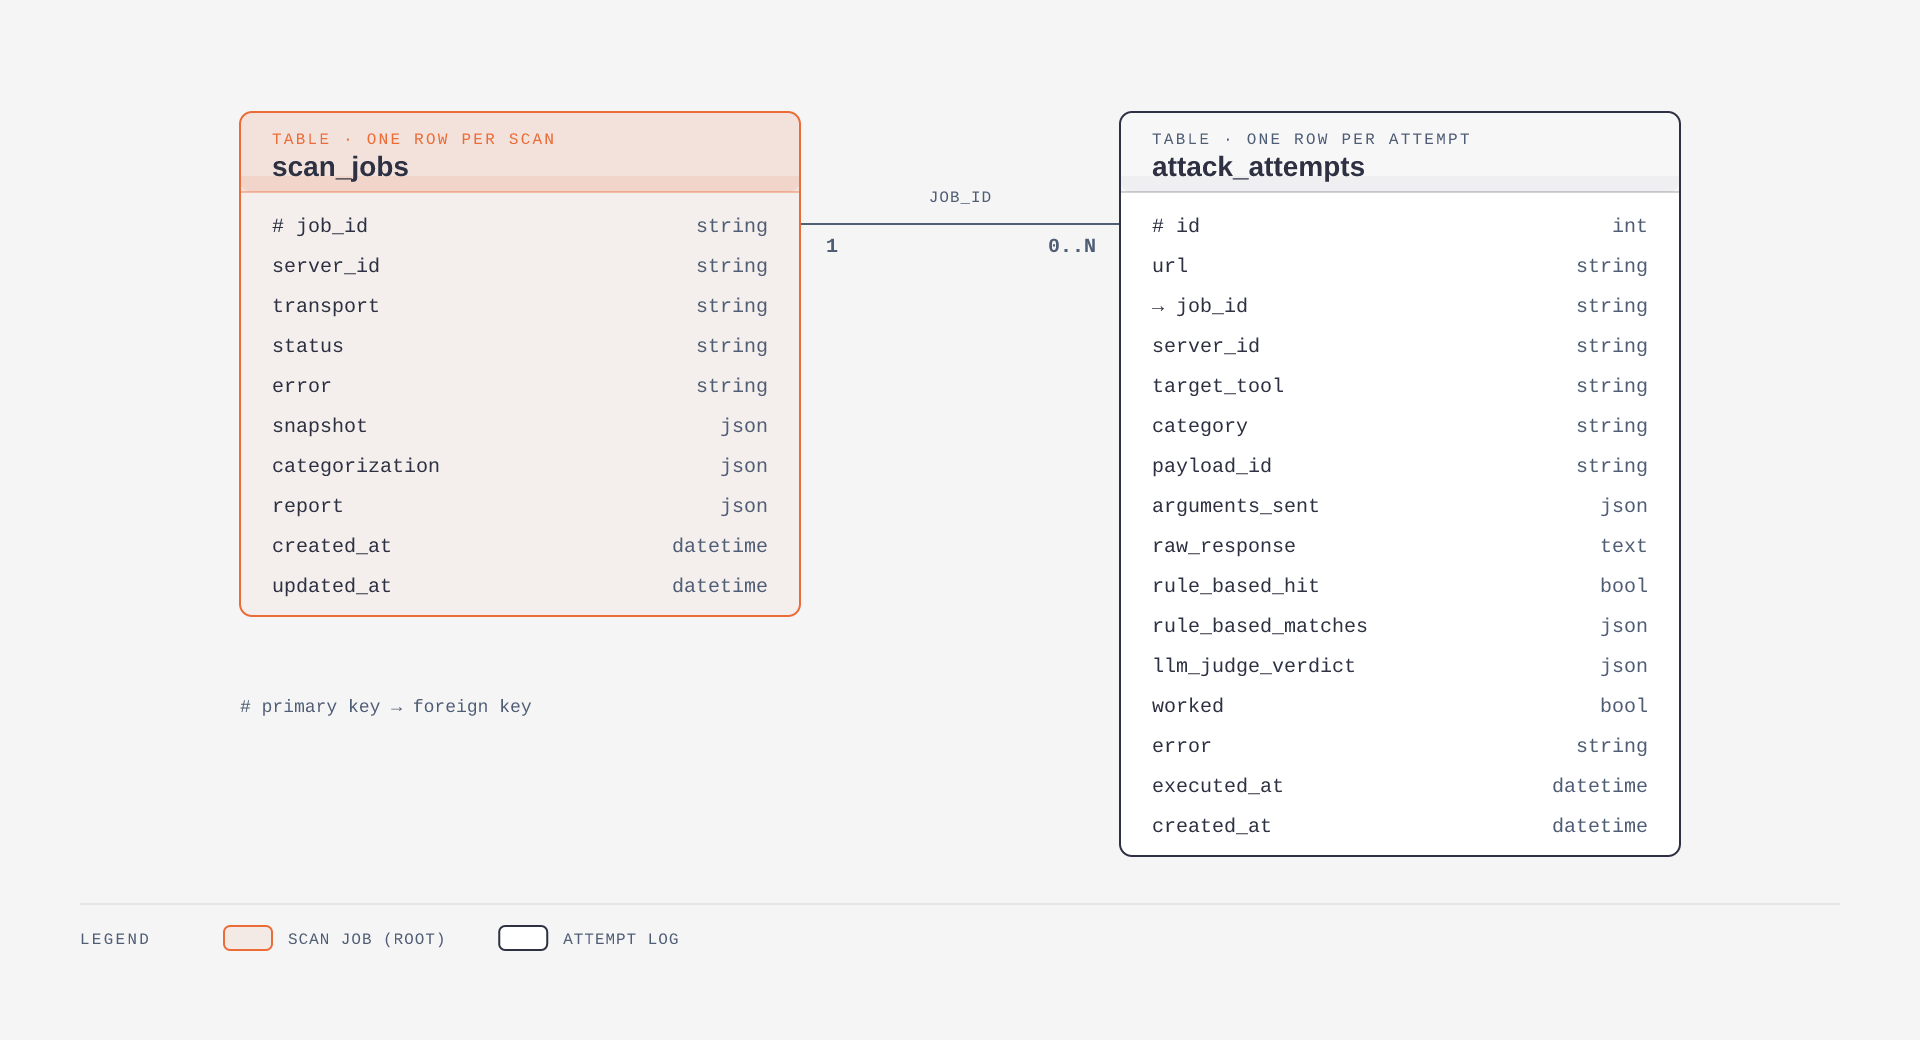
\includegraphics[width=\linewidth]{images/arch-data-model.png}
    \caption{Persisted data model. Only scan outputs are stored; connection credentials never are.}
    \label{fig:data-model}
\end{figure}

What the model deliberately does not store is the connection credentials. The \acrshort{url}, headers, or command used to reach the target, which may carry a bearer token for the server under test, live only in memory for the duration of one discover-then-attack cycle and are deleted as soon as the attack run finishes. The cost of this choice is that a process restart between discovery and attack forces a fresh discovery; the benefit is that a security tool never becomes a store of the very credentials it was handling. This is examined further in the next section.

\section{Architectural Design Decisions}
\label{sec:decisions}

Several choices shape the architecture rather than any single component, and each answers a question a reviewer would reasonably raise.

Discovery and attack are two separate operations. The read-only discovery call never sends attack traffic, and the attack call refuses to run without the identifier of a prior discovery. This is the structural form of the \glsdisp{human_in_the_loop}{human-in-the-loop} gate: nothing is attacked without a deliberate second action, taken after the operator has seen the full categorization.

Connection credentials are never persisted. As described in Section~\ref{sec:data}, only scan outputs reach the database. For a security tool specifically, the risk of accumulating target credentials outweighs the convenience of surviving a restart.

Evaluation is dual rather than single. Rule-based checks are fast, precise, and free, but blind to anything that does not match a known format. The \gls{llm} judge catches the semantic leaks no regular expression could enumerate in advance, at the cost of one extra model call, and it runs only where that cost is justified. Crucially, the judge's verdict is grounded, not trusted: it must quote the exact span of the response that proves the finding, and a verdict whose evidence cannot be located in the response is overruled. This guard is deterministic and independent of which model is configured, so it catches a confidently wrong judge regardless of provider.

Severity comes from a public standard rather than from the judge. The \gls{llm} judge decides whether an attack succeeded and how confident it is, but the severity of a confirmed finding is the band of its category's \gls{cvss} vector (Section~\ref{sec:scoring}). Letting the model also choose the severity would put a second unvalidated judgement in the report, one that could differ between runs and providers for the same evidence. Fixing it to the standard makes every finding of the same category comparable across servers, scans, and models. The same reasoning sets the single aggregate figure for a scan: the highest \gls{cvss} score among its findings, which is the usual convention in vulnerability reporting: the worst confirmed weakness decides how exposed the server is.


Classification uses a System One model rather than a generative \gls{llm}. The tool was first built with an \gls{llm} classifier, which is kept in the code for comparison. Classification is a narrow decision, repeated for every tool and category and consumed by code rather than read by a person, which is the case a System One model is built for: each category becomes an independent probability that can be thresholded, instead of a list the model writes and the code must parse. In a benchmark over the 22 tools of the evaluation corpus (Chapter~\ref{chap:results}), Jev reached an F1 score of 0.86, against 0.84 and 0.86 for the \gls{llm} classifier (GPT-5.4 mini) in two runs, at roughly one seventh of the cost and less than half of the latency per tool. Attack synthesis and judging stay with a generative \gls{llm}, because they require writing text and explaining a verdict.

The classifier has a floor it cannot remove. Because a tool description is untrusted text fed into a model, a crafted description could try to manipulate the classifier into reporting nothing. Each Jev question therefore instructs the model to treat the tool definition as data rather than instructions, the application adds the generic-fuzzing floor to every result whatever the model answers, and a tool whose classification fails falls back to that baseline instead of being dropped. Together these ensure that no tool silently vanishes from the results. The tool's own triage step is exposed to the same injection risk it is built to detect, and the architecture answers that explicitly rather than assuming the classifier is trustworthy.

Attacks run sequentially by default. A strictly sequential run is deterministic and reproducible, which is the right baseline for any measurement. Parallelism is available on request for speed, but it changes the order and the load, not the set of findings, and timing-sensitive checks are always isolated so that scan-induced load cannot corrupt a latency-based verdict.
